%preamble
\documentclass[letterpaper]{article}
\synctex=1

\usepackage{geometry}
\usepackage{array}
\usepackage{lipsum}

\usepackage{graphicx}
\usepackage{float}
\graphicspath{ {images/} }

\usepackage[hidelinks]{hyperref}

\usepackage{xcolor}
\usepackage[utf8]{inputenc}
% \usepackage[section]{placeins}
%
% \newenvironment{changemargin}[2]{%
% \begin{list}{}{%
% \setlength{\topsep}{0pt}%
% \setlength{\leftmargin}{#1}%
% \setlength{\rightmargin}{#2}%
% \setlength{\listparindent}{\parindent}%
% \setlength{\itemindent}{\parindent}%
% \setlength{\parsep}{\parskip}%
% }%
% \item[]}{\end{list}}

% \usepackage{tabu}
%actual document

\renewcommand{\thesection}{Task \arabic{section}}


\begin{document}

%titlepage
\begin{titlepage}
 \begin{center}

  \LARGE
  ECE 321 Lab\\ Software Requirements Engineering

  Department of Electrical and Computer Engineering\\

  University of Alberta

  \vspace{2cm}

  Lab Report \# 4: Intro to Petri Nets

  \vspace{2cm}

  Team Name: 404 Team Name Not Found

  \vspace{2cm}

  \today

  \vspace{2cm}
  \Large

  \begin{tabular}{ | m{5cm} | m{5cm} | }
   \hline
   Student Name  & Student \\
   \hline
   Arun Woosaree & XXXXXX  \\
   \hline
   Liyao Jiang   & XXXXXX  \\
   \hline
   Zhi Shen      & XXXXXX  \\
   \hline
  \end{tabular}



 \end{center}
\end{titlepage}

%%table of contents
% \tableofcontents
% \vfill
% \newpage

\section{}

\textit{Generate all possible states, in the format (P0, P1, P2) for the Petri Net shown below. Can this network run infinitely long?}

\begin{figure}[H]
 \centering
 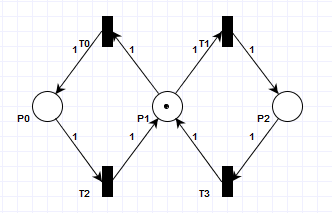
\includegraphics[width=\textwidth]{image1.png}
 % \caption{}
\end{figure}

The states are as follows:

\begin{itemize}
 \item S1(1,0,0)
 \item S2(0,1,0)
 \item S3 (0,0,1)
\end{itemize}

Net 1 can run infinitely, because it does not have a deadlock and all the states
are vanashing.

\textit{Modify the network to the below setting, and again generate all possible states. Explain why these states are different from states generated above (use proper terminology, such as predicates, places, tokens, firing, and transitions). Can this network run infinitely long, and if not what are the end-states?
 Note that arcs have numbers on them, and there is a different initial marking.
}

\begin{figure}[H]
 \centering
 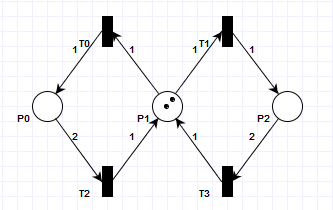
\includegraphics[width=\textwidth]{image2.png}
 % \caption{}
\end{figure}

\section{}

\textit{Build a semaphore network with the below initial marking, as shown below. Process 1 is denoted on the left, and process 2 on the right.
}
\begin{figure}[H]
 \centering
 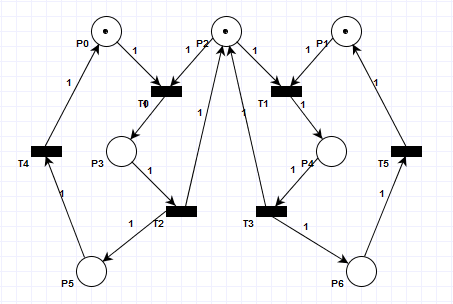
\includegraphics[width=\textwidth]{image3.png}
 % \caption{}
\end{figure}

\textit{Answer the following questions:}

\subsection{}
\textit{Enumerate all states of the semaphore in the (P0, P1, P2, P3, P4, P5, P6) format.Hint: you can use "Analysis Module Manager $\rightarrow$ Reachability/Coverability Graph" option.
}

\subsection{}
\textit{Which of the states represent a situation when process 1 OR process 2 take possession of the shared resource?}\\

\textbf{WTF IS THIS?}

\subsection{}
\textit{Is it possible to reach state (0, 0, 0, 1, 1, 0, 0)? What does this state represent?}

\section{}

\begin{figure}[H]
 \centering
 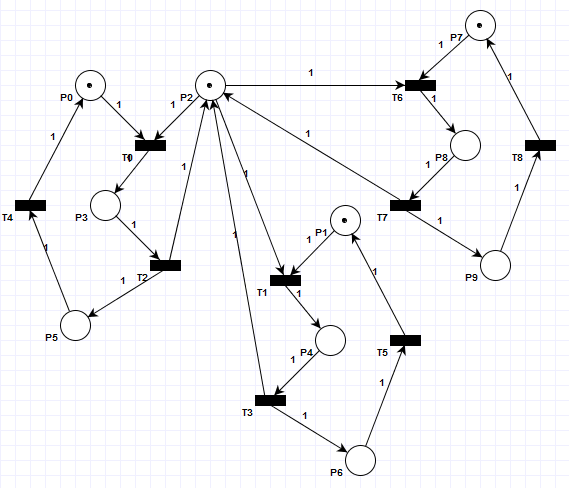
\includegraphics[width=\textwidth]{image4.png}
 % \caption{}
\end{figure}

\textit{Answer the following questions:}

\subsection{}
\textit{How many states does this network have?
}\\

This network has 23 states.

\subsection{}
\textit{Which places are responsible for showing if a given process has access to the shared resource?}

\subsection{}
\textit{Is it possible that this network will have more than 4 OR less than 3 tokens in any possible state?
 If yes, then list these states.
}

\subsection{}
\textit{Generate four starvation cycles for this network. Represent the cycles in terms of the firing sequences. Is it possible to have more than 4 starvation cycles for this network?}

\subsection{}
\textit{Modify the 3 processes semaphore model to the below one, including the initial marking.
 Note that some arcs have numbers on them, and there is a different initial marking.
}

\begin{figure}[H]
 \centering
 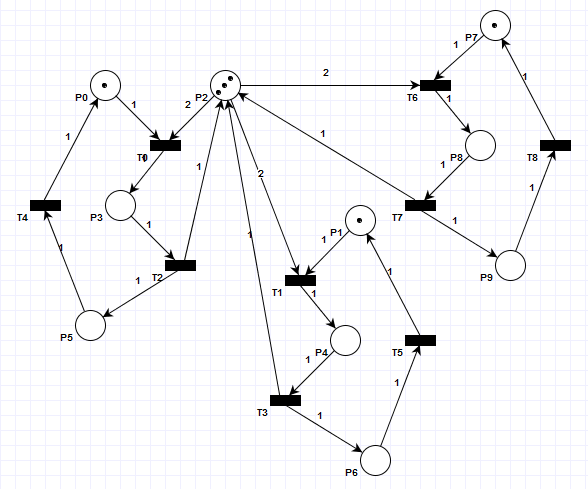
\includegraphics[width=\textwidth]{image5.png}
 % \caption{}
\end{figure}

\textit{Is it possible that two processes will be able to access the shared resource at the same time in the above model? If yes, then give the state that shows this situation.}

\vspace{2cm}
\textit{Is the number of tokens bounded in this network (is it possible to have a place that may have continuously increasing number of tokens)? If yes, then what is the maximum number of tokens in the network? Also, in this case list all the states in which the maximum number of tokens occurs.
 Use the (P0, P1, P2, P3, P4, P5, P6, P7, P8, P9) format
}


\vspace{1cm}
\textit{What is the minimum number of tokens in the above network?}

\section{}

\textit{Start by loading and compiling the two semaphores network model created in TASK 2. Use the “Analysis module manager” section.}

\subsection{}
\textit{Perform the state enumeration with initial marking (1, 1, 1, 0, 0, 0, 0), and answer the following questions}

\subsubsection{}
\textit{How many reachable states are there for this network and initial marking?}

\subsubsection{}
\textit{How many places in this network never receive any tokens, how many receive a single token, and how many receive more than one token}

no tokens: \\
single token: \\
more than one token: \\

\subsubsection{}
\textit{Explain what does it mean that a network is strictly conservative}

\subsubsection{}
\textit{Does the network have any deadlocks, is it bounded and safe?}

\subsubsection{}
\textit{List all t-invariants of the network.}

\subsection{}
\textit{Perform the state enumeration with initial marking (2, 0, 2, 0, 0, 0, 0), and answer the following questions.}

\subsubsection{}
\textit{Which transitions can be fired in state S2 (1, 0, 2, 0, 0, 1, 0)?}

\subsubsection{}
\textit{List all the reachable states in the (P0, P1, P2, P3, P4, P5, P6) format}

\subsubsection{}
\textit{How many places in this network never receive any tokens, how many receive a single token, and how many receive more than one token}

no tokens: \\
single token: \\
more than one token: \\


\section{}

Screenshots of the lab VM for each of the group members:

\begin{figure}[H]
 \centering
 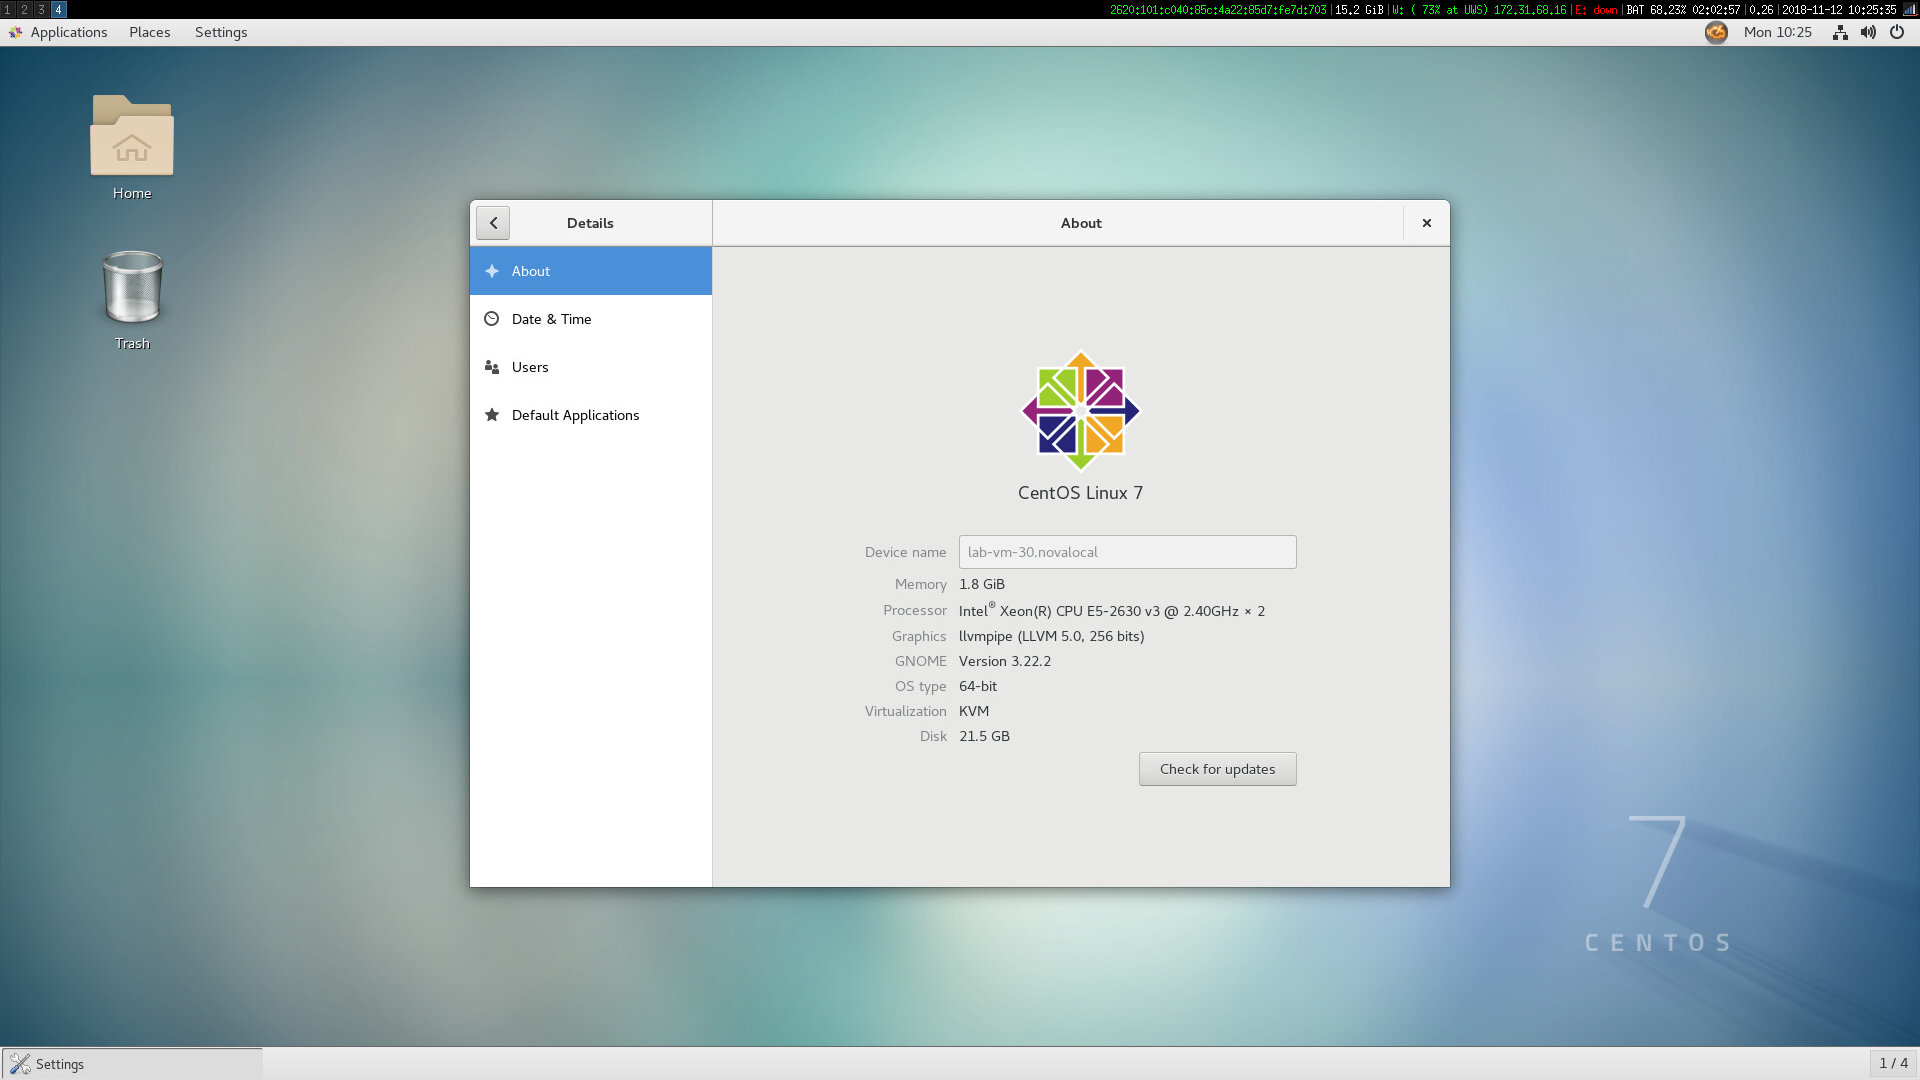
\includegraphics[width=\textwidth]{arun.png}
 \caption{Arun Woosaree}
\end{figure}

\begin{figure}[H]
 \centering
 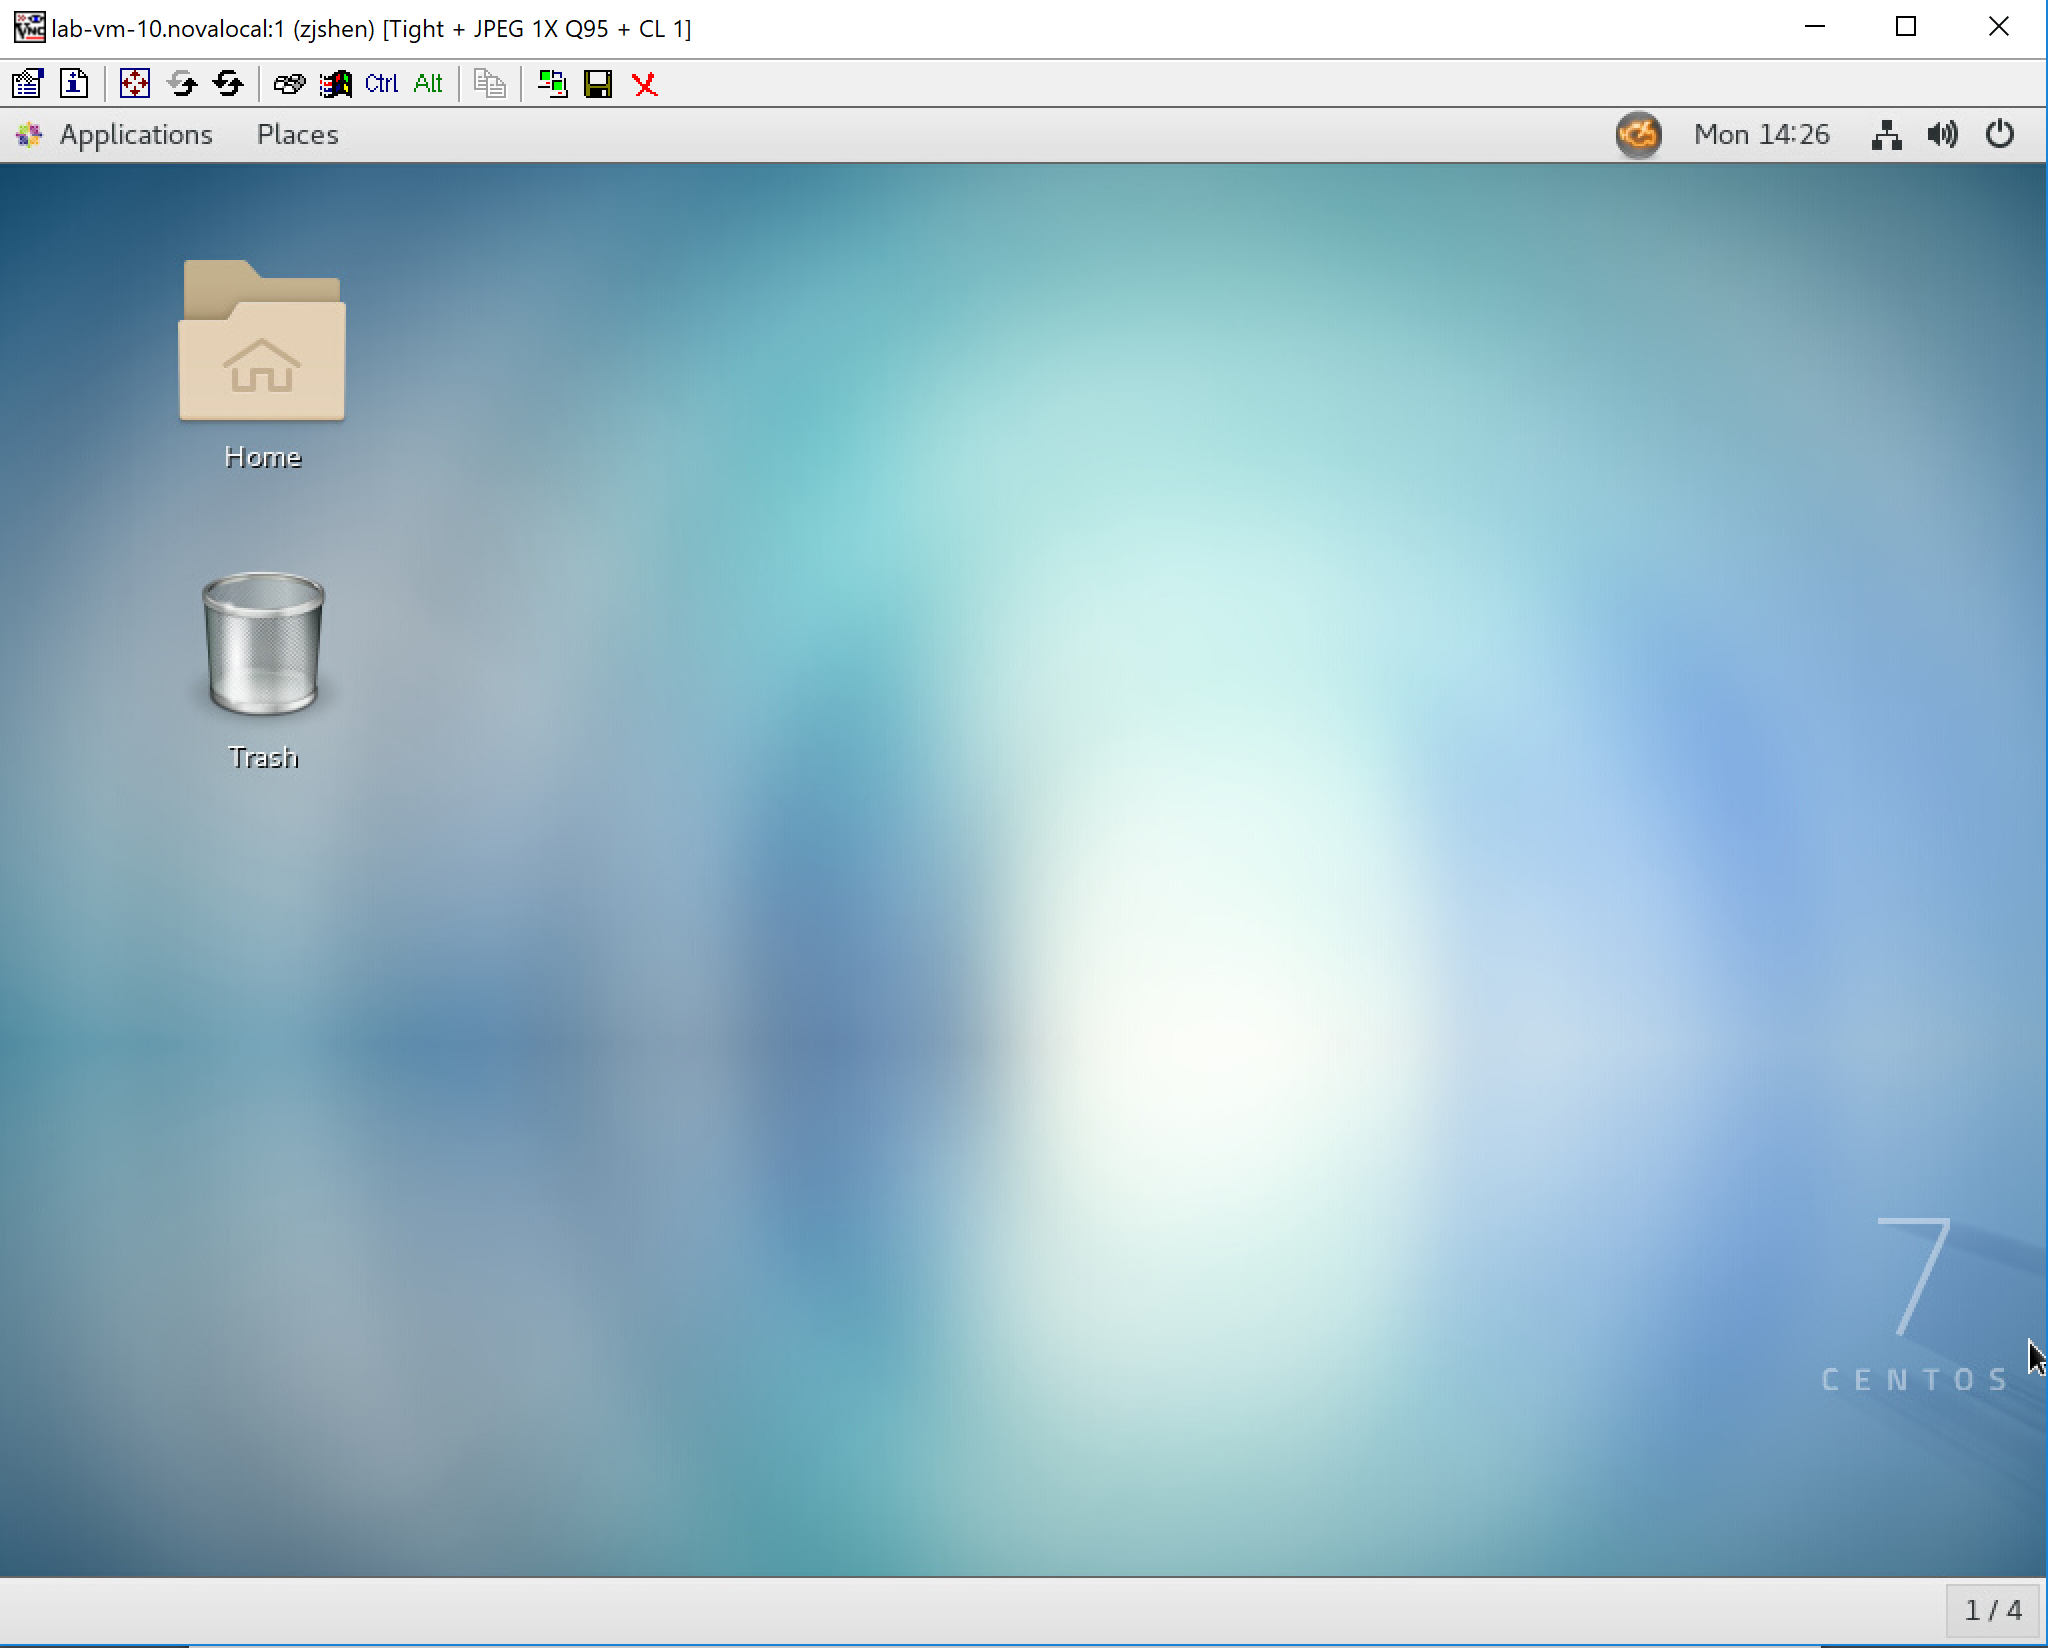
\includegraphics[width=\textwidth]{max.png}
 \caption{Zhi Shen}
\end{figure}

\begin{figure}[H]
 \centering
 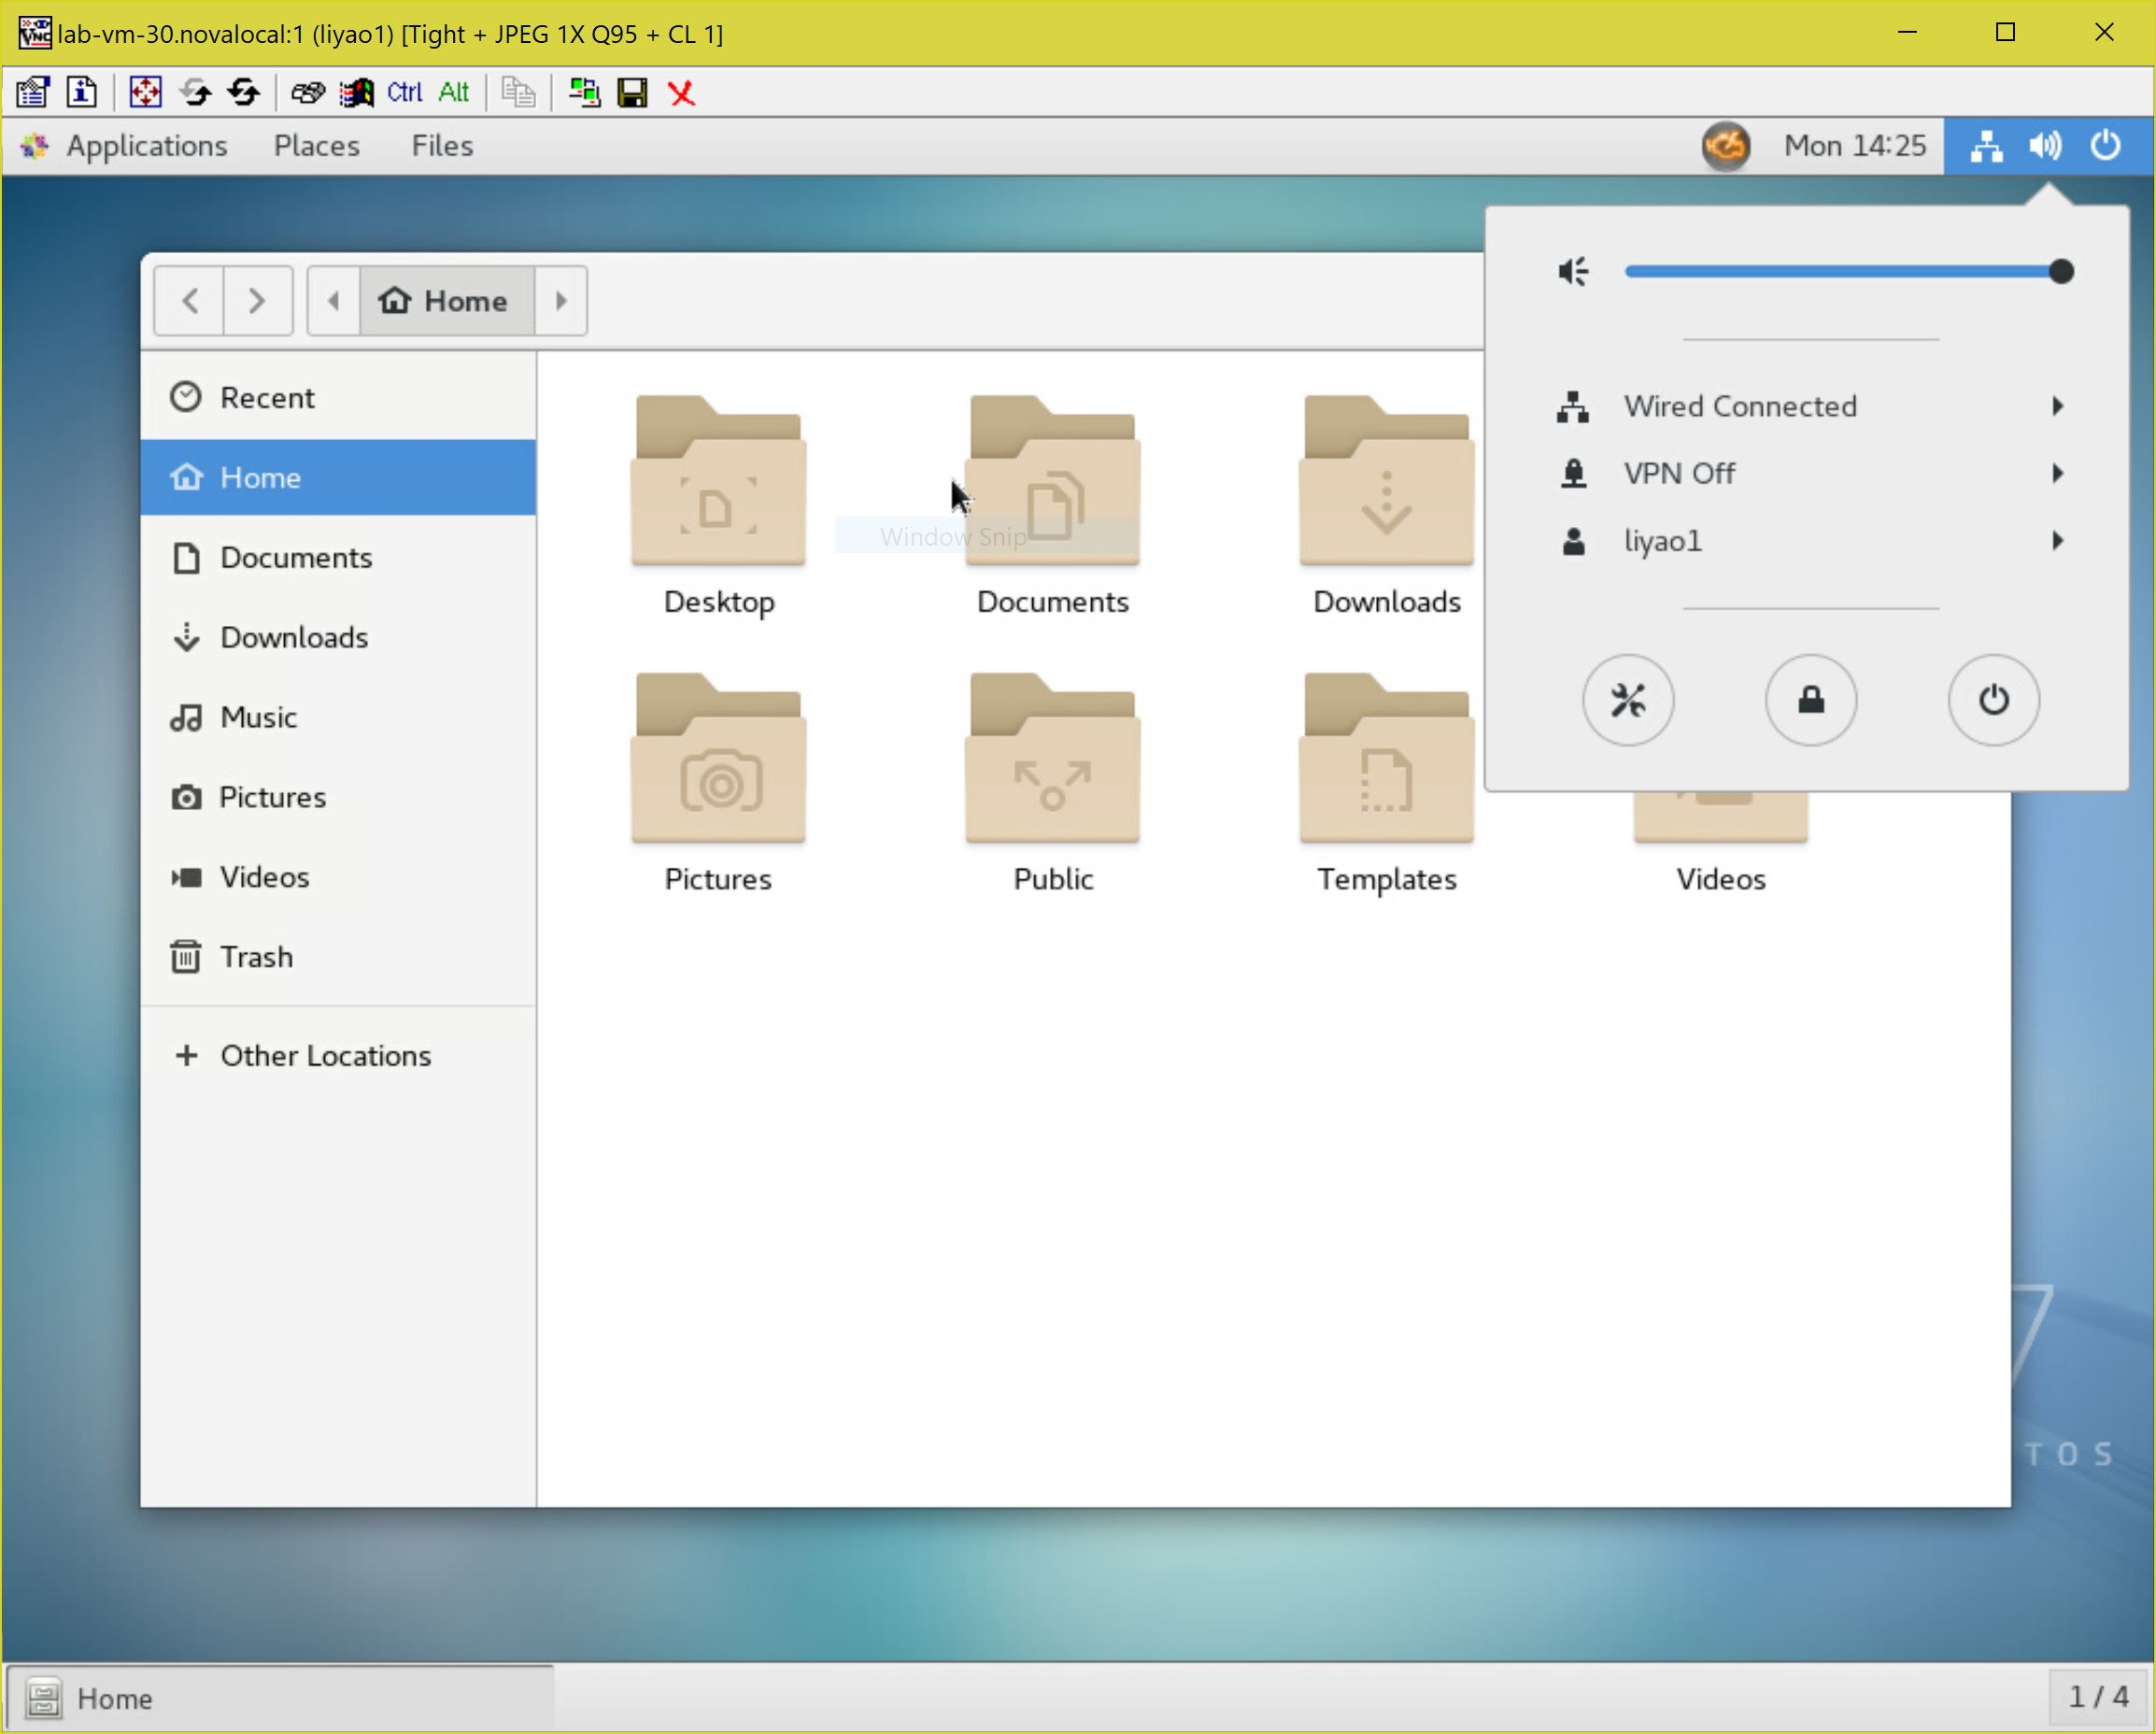
\includegraphics[width=\textwidth]{liyao.jpg}
 \caption{Liyao Jiang}
\end{figure}

\end{document}
